\section{Chilled water (CW) loop}\label{chilled-water-cw-loop}

The chilled water loop is constructed by using a \emph{PlantLoop} object\emph{.} This loop uses a water-cooled electric chiller to supply chilled water to the demand side of this loop. As mentioned above, the cooling coil is replaced by a load profile object that contains the demand load profile. The chiller is operated by using set points, plant equipment operation schemes and schedules. Refer to Figure~\ref{fig:simple-line-diagram-for-the-chilled-water} for a simple diagram of the Chilled Water Loop.

\begin{figure}[hbtp] % fig 15
\centering
\includegraphics[width=0.9\textwidth, height=0.9\textheight, keepaspectratio=true]{media/image015.png}
\caption{Simple line diagram for the chilled water loop \protect \label{fig:simple-line-diagram-for-the-chilled-water}}
\end{figure}

\subsection{Flowcharts for the CW Loop Input Process}\label{flowcharts-for-the-cw-loop-input-process}

This series of flow charts serve as a process guide for identifying and inputting the chilled water loop and its components into the input file. Refer to Figure~\ref{fig:energyplus-line-diagram-for-the-chilled-water} for an EnergyPlus schematic of the Chilled Water Loop.

\begin{figure}[hbtp] % fig 16
\centering
\includegraphics[width=0.9\textwidth, height=0.9\textheight, keepaspectratio=true]{media/image016.png}
\caption{EnergyPlus line diagram for the chilled water loop \protect \label{fig:energyplus-line-diagram-for-the-chilled-water}}
\end{figure}

The ``PlantLoop'' object is entered into the input file, with water as the working fluid. The supply side of the chilled water loop is then input into the system followed by the demand side. A flow chart for separating the half loops in the loop is provided in Figure~\ref{fig:simple-flowchart-for-separation-of-half-loops}.

\begin{figure}[hbtp] % fig 17
\centering
\includegraphics[width=0.9\textwidth, height=0.9\textheight, keepaspectratio=true]{media/image017.png}
\caption{Simple flowchart for separation of half loops in the chilled water loop \protect \label{fig:simple-flowchart-for-separation-of-half-loops}}
\end{figure}

\subsubsection{CW Loop Supply Side Loop Construction}\label{cw-loop-supply-side-loop-construction}

The main components in the supply side of the chilled water loop are the circulation pump for the chilled water and the electric chiller that supplies the chilled water. The set-point is set to the outlet node of this half of the loop; the temperature at this node is controlled to regulate the operation of the chiller. This side of the loop has eight nodes, four components and four branches, while it is not required to define individual node positions in the loop, the components and branches have to be defined with an inlet and an outlet node. Connectors are the objects that connect the branches together and complete the loop. Therefore, the branches and the connectors will set the positions of the nodes in the loop. The EnergyPlus line diagram for the Chilled Water Loop supply side is provided in Figure~\ref{fig:energyplus-line-diagram-for-the-supply-side}. The flowchart for supply side branches and components is provided in Figure~\ref{fig:flowchart-for-chilled-water-loop-supply-side-and}. The flowchart for the supply side connectors is provided in Figure~\ref{fig:flowchart-for-chilled-water-loop-supply-side-connectors}.

\begin{figure}[hbtp] % fig 18
\centering
\includegraphics[width=0.9\textwidth, height=0.9\textheight, keepaspectratio=true]{media/image018.png}
\caption{EnergyPlus line diagram for the supply side of the chilled water loop \protect \label{fig:energyplus-line-diagram-for-the-supply-side}}
\end{figure}

\begin{figure}[htbp] % fig 19
\centering
\includegraphics{media/image019.png}
\caption{Flowchart for chilled water loop supply side branches and components \protect \label{fig:flowchart-for-chilled-water-loop-supply-side-and}}
\end{figure}

\begin{figure}[htbp] % fig 20
\centering
\includegraphics{media/image020.png}
\caption{Flowchart for chilled water loop supply side connectors \protect \label{fig:flowchart-for-chilled-water-loop-supply-side-connectors}}
\end{figure}

\subsubsection{CW Loop Demand Side Loop Construction}\label{cw-loop-demand-side-loop-construction}

The demand side of the loop is entered next. The main component in this side of the loop is the cooling load profile(instead of the cooling coil). This load profile is input by using a Schedule:Compact object which indicates the hourly cooling loads for the annual run period. In a more general scenario a cooling coil would take the place of the load profile and the cooling load will be simulated from the data obtained in the building system energy simulation. Apart from the load profile, the structure of the loop is very similar to the structure of the supply side. This side of the loop also has eight nodes, four components, and four branches. An EnergyPlus schematic for the demand side is provided in Figure~\ref{fig:energyplus-line-diagram-for-the-demand-side}. The flowchart for demand side branch definition is provided in Figure~\ref{fig:flowchart-for-chilled-water-loop-demand-side-and}. The flowchart for the demand side connectors is provided in Figure~\ref{fig:flowchart-for-chilled-water-loop-demand-side-connectors}.

\begin{figure}[htbp] % fig 21
\centering
\includegraphics{media/image021.png}
\caption{EnergyPlus line diagram for the demand side of the chilled water loop \protect \label{fig:energyplus-line-diagram-for-the-demand-side}}
\end{figure}

\begin{figure}[htbp] % fig 22
\centering
\includegraphics{media/image022.png}
\caption{Flowchart for chilled water loop demand side branches and components \protect \label{fig:flowchart-for-chilled-water-loop-demand-side-and}}
\end{figure}

\begin{figure}[htbp] % fig 23
\centering
\includegraphics{media/image023.png}
\caption{Flowchart for chilled water loop demand side connectors \protect \label{fig:flowchart-for-chilled-water-loop-demand-side-connectors}}
\end{figure}

As shown in the flowchart above, the load profile is attached to the chilled water loop at its designated position (the LoadProfile:Plant object can be used just like any other component) on the demand side of the loop.

\subsection{Flowcharts for CW Loop Controls}\label{flowcharts-for-cw-loop-controls}

The chilled water loop is operated by using set-points, plant equipment operation schemes and schedules.

\subsubsection{Chilled Water Loop Schedules}\label{chilled-water-loop-schedules}

The chilled water loop uses two different schedules to operate properly. The \emph{Chiller AlwaysOnSchedule} is a compact schedule that keeps the chiller ON at all times of the day for a whole year. This compact schedule uses a discrete \emph{ScheduleTypeLimit} (\emph{CW Loop On/Off)} which defines that the value of On is 1 and that of Off is 0. This plant loop also uses another compact schedule named \emph{CW Loop Temp Schedule} to set the temperature at the chilled water loop outlet node. This schedule uses a schedule type limit named \emph{CW Loop Any Number}. The flowchart for chilled water loop schedule definition is provided in Figure~\ref{fig:flowchart-for-chilled-water-loop-schedules}.

\emph{~}

\begin{figure}[htbp]
\centering
\includegraphics{media/image024.png}
\caption{Flowchart for chilled water loop schedules \protect \label{fig:flowchart-for-chilled-water-loop-schedules}}
\end{figure}

\subsubsection{Chilled Water Loop Plant Equipment Operation Schemes}\label{chilled-water-loop-plant-equipment-operation-schemes}

The \emph{PlantEquipmentOperationschemes} object uses the \emph{Chiller AlwaysOnSchedule} and the \emph{CW Loop Cooling Load} objects to set the range of the demand load for which the chiller can be operated during the simulation period. Operation schemes are especially useful and crucial when using multiple active components. For example, the performance of multiple chillers can be optimized by carefully managing the load ranges on each of the chillers. A flowchart detailing the chilled water loop plant equipment operation schemes is provided in Figure~\ref{fig:flowchart-for-chilled-water-loop-plant-equipment}.

\begin{figure}[htbp]
\centering
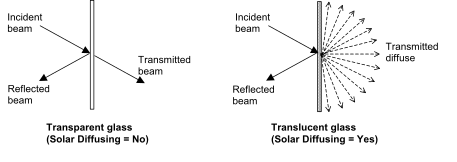
\includegraphics{media/image025.png}
\caption{Flowchart for chilled water loop plant equipment operation schemes \protect \label{fig:flowchart-for-chilled-water-loop-plant-equipment}}
\end{figure}

\subsubsection{Chilled Water Loop Setpoints}\label{chilled-water-loop-setpoints}

The \emph{Chilled Water Loop Setpoint Manager} uses the \emph{CW Loop Temp Schedule} to set a temperature control point at the \emph{CW Supply Outlet Node}. This setpoint allows the program to control the temperature at the node by operating the components in the chilled water loop. ~Since, setpoint managers are high-level control objects, their usefulness is realized in much more complex systems, where multiple nodes have to be monitored in order to operate the system properly. A flowchart for chilled water loop setpoints is provided in Figure~\ref{fig:flowchart-for-chilled-water-loop-setpoints}.

\begin{figure}[htbp]
\centering
\includegraphics{media/image026.png}
\caption{Flowchart for chilled water Loop setpoints \protect \label{fig:flowchart-for-chilled-water-loop-setpoints}}
\end{figure}

\subsubsection{Chilled Water Loop Sizing}\label{chilled-water-loop-sizing}

The chilled water loop is sized such a way that the design loop exit temperature is 7 degrees Celsius, and the loop design temperature difference is 5 degrees Celsius. A flowchart for the chilled water loop sizing is provided in Figure~\ref{fig:flowchart-for-chilled-water-loop-sizing}. Note: Since the Load Profile object does not demand any feedback from the \emph{PlantLoop} object, the chilled water loop does not necessarily need to be sized (This object is commented out in the example file). The sizing shown here is just an example of how the object class can be used in EnergyPlus.

\begin{figure}[htbp]
\centering
\includegraphics{media/image027.png}
\caption{Flowchart for chilled water loop sizing \protect \label{fig:flowchart-for-chilled-water-loop-sizing}}
\end{figure}
